\newpage
\chapter{Moment of Inertia}
\label{mt:c:Appendix}
\label{mt:c:Appendix:s:Moment of inertia}

The physical modelling and simulation of a rigid body needs to be described with
the dynamic behaviour of that. So the quadrocopter \gls{UAV} can be described with the
\gls{EOM} described in chapter \ref{mt:c:literature:s:equations_of_motion} in
relation to the moment inertias, which describe the resistance of the \gls{UAV} rigid body against changes in rotational
directions. Such moment inertia is described as a \ensuremath{3x3} matrix, also
called tensor, for a rigid body with 6 \gls{DOF}. The assumption that the B-frame originates in the
point of mass of the quadrocopter \footnote{See chapter
\ref{fig:QuadrocopterPhysicalModel}},
 simplifies \ensuremath{I}, to a matrix with just diagonal entries \ensuremath{(Ixx,
 Iyy, Izz)}\footnote{The moment inertia matrix and the
 corresponding pictures are derived from \citebib[pp.24
-33 Determination of the moment of inertia]{SchSunVetWebFriSat10}}.

\begin{equation}
\label{formula:InertiaMatrix}
I=\begin{pmatrix} I_{XX} & I_{XY} & I_{XZ} \\ I_{YX} & I_{YY} & I_{YZ} \\ I_{ZX}
& I_{ZY} & I_{ZZ} \end{pmatrix} =  
\begin{pmatrix} I_{XX} & 0 & 0 \\ 0 & I_{YY} & 0 \\ 0 & 0 & I_{ZZ} \end{pmatrix}
\end{equation} 

% For determination of the inertia either a measurement can be performed by using a
% rotary table or it can be calculated by substituting the real parts of the
% quadrocopter with simplified parts like cylinders or blocks. In this project the
% second approach was used. Thereby the quadrocopter model was abstracted in the
% structure shown in figure ...
% 
% This structure contains:
% 
% \begin{itemize}
% 
% \item One hemisphere:
% The hemisphere substitutes all the electronic parts (flight control,
% brushless controller, parts of the wiring harness and the construction plates)
% 
% A hemisphere is given by its radius r, see \ref{}. The centre of gravity is
% located above the flattened part of the hemisphere. The inertias around the
% z-axis and around the other axes parallel to the flat part of the hemisphere are
% computed as shown in equation \ref{}.
% \item :
% 
% \end{itemize}
% 


\chapter{Mathematical Description of Distortions}
\label{mt:c:Appendix:Mathematical_description_of_distortions}
Distortions can occur if the distance of image points to the centre of projection
varies, or if the centre of projection is not in the centre of the image. These
kinds of distortions are defined as radial \ensuremath{x_dr, y_dr} and decentring
\ensuremath{x_dd, y_dd} distortions, and represent the components of the complete
distortion of images \ensuremath{x_d, y_d}.

The following formulas\footnote{This formulas are derived from the formulas
presented in \citebib[p.30 Mathematical description of distortions]{Fac08}}
describe the possible distortions of images and show that the complexity of an
image equalisation is proportional to the image points e.g. the image dimensions.
Thereby the values \ensuremath{x_n, y_n} describe a point of an image, which has
to be equalized. The distance radius to the centre of the image
\ref{formula:r_x_n_y_n} is a important component and is used in combination of
the distortion coefficients \ensuremath{ k_{cn} : n \in \{1, 2, 3,
4, 5 \}} to eliminate the mentioned components of distortion.


\begin{equation}
\label{formula:x_d_y_d}
\begin{array}{l}
x_d = x_{dr} + x_{dd} \\
y_d = y_{dr} + y_{dd}
\end{array}
\end{equation}

\begin{equation}
\label{formula:r_x_n_y_n}
\begin{array}{l}
r = \sqrt(x_n^2+y_n^2)
\end{array}
\end{equation}

\begin{equation}
\label{formula:x_dr_y_dr}
\begin{array}{l}
x_{dr} = (1+k_{c1}*r^2+k_{c2}*r^4+k_{c5}*r^6)*x_n\\
y_{dr} = (1+k_{c1}*r^2+k_{c2}*r^4+k_{c5}*r^6)*y_n
\end{array}
\end{equation}

\begin{equation}
\label{formula:x_dd_y_dd}
\begin{array}{l}
x_{dd} = 2*k{c3}x_n*y_n+k_{c4}*(r^2+2*x_{n}^2)\\
y_{dd} = k_{c3}*(r^2+2*y_{n}^2)+2*k_{c4}*x_{n}*y_{n}
\end{array}
\end{equation}


These calculations can be executed initial for the camera calibration, and
further for the real-time equalization for the trajectory movement of the camera.
Popular calibration processes transform the distortions to a value in which, 
can be considered as equalised. Such a calibration process is described by Tsai
 et al. \citebib[Camera Calibration by Tsai]{TsaLen89} and extended by Zhang
 \citebib[Visual Servoing with Dynamics]{ZhaOst99}, and describes an iterative way
 for the determination of the coefficients \ensuremath{k_{cn}}. Thereby a
 squared image is used as reference for the camera and the algorithm, described in figure
 \ref{fig:EqualizationAlgorithm.png}\footnote{This picture extends the scheme
 picture presented in \citebib[p.32 Equalization of a captured image]{Fac08}}, is
 executed iteratively. Real-time equalisation processes mostly are implemented
 with an array of distortion coefficients and can effective determine these with
 a lookup  operation\footnote{See, Distortion Correction with FPGA \citebib[pp.
 System Design]{GriJohBai03}}.


\begin{figure}[H]
	\centering
		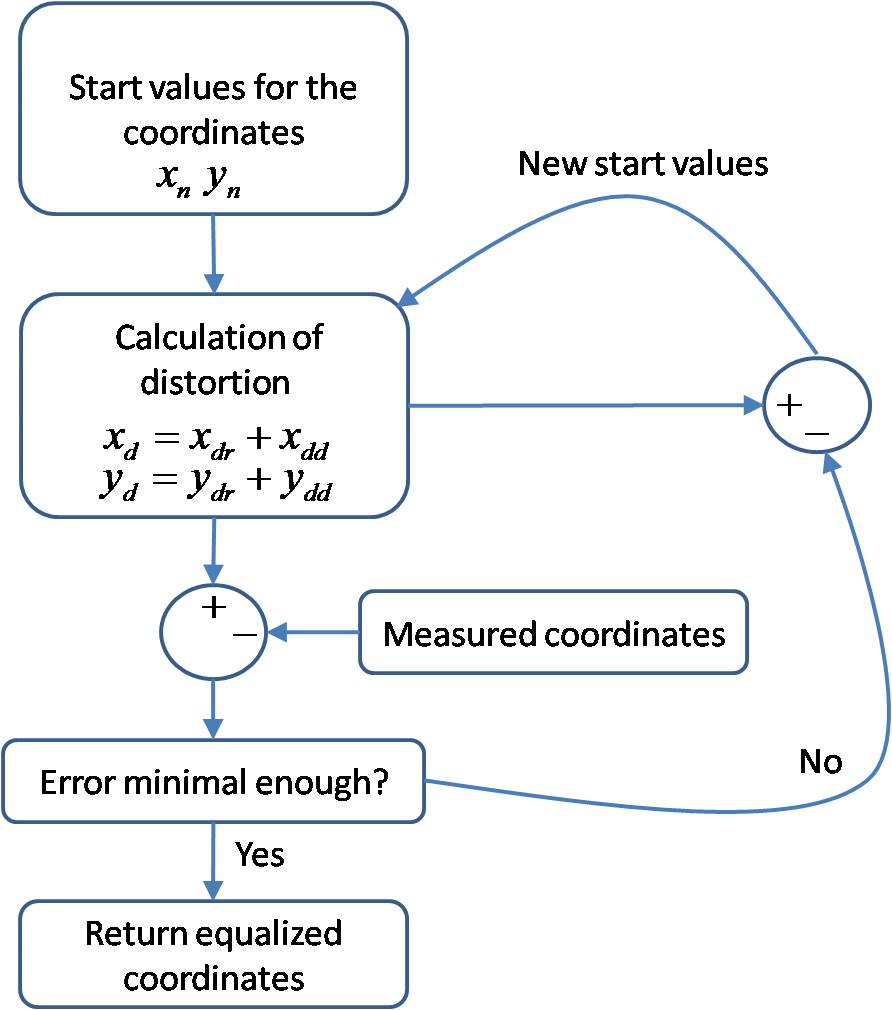
\includegraphics[width=0.75\textwidth, height=0.75\textwidth]{graphic/EqualizationAlgorithm.png}
\caption{Equalization algorithm of distorted images}
	\label{fig:EqualizationAlgorithm.png}
\end{figure}


\chapter{Characteristics of Sensor Noise}
\label{mt:c:Appendix:s:Characteristics of Sensor Noise}

The captured sensor noise of the \gls{IMU} can be characterized with the sample variance of the 
readout random sample. Thereby the Bias-corrected Sample Variance(\gls{sym_BCSV}) (See \ref{formula:BCSV})
 can be used to determine the variance of a random set of values. This variance can be used as 
characteristic for noise generators, as well it was used in focus of this projects' simulation.

\begin{equation}
\label{formula:BCSV}
S^{2}_{N-1} = \frac{1}{N-1}*\sum\limits_{i=1}^N (x_i -  \bar{x}^2)
\end{equation}

The derived \gls{sym_BCSV} values are presented in table \ref{table:BCSVs}. These values are derived from a list
of measures captured over 11 seconds in an interval of 100 milliseconds.
\begin{figure}
\begin{table}[H]
\centering
\begin{tabular}{|l|l|l|l|l|l|}
\hline
\ensuremath{S^{2}_{N-1}(\ddot x_e)} & \ensuremath{S^{2}_{N-1}(\ddot y_e)} & \ensuremath{S^{2}_{N-1}(\ddot z_e)} & \ensuremath{S^{2}_{N-1}(p)
~Roll} & \ensuremath{S^{2}_{N-1}(q)~Pitch} & \ensuremath{S^{2}_{N-1}(r)~Yaw}\\
\hline
\hline
2.178 \ensuremath{m/s^2} & 0.576 \ensuremath{m/s^2} & 6.860 \ensuremath{m/s^2} & 0.003 \ensuremath{rad/s} & 0.001 \ensuremath{rad/s} & 0.001 \ensuremath{rad/s}\\
\hline
\end{tabular}
\end{table}
\caption{Derived Bias-corrected sample variances of sensor captured values}
\label{table:BCSVs}
\end{figure}


\chapter{Image Processing Test Scenario Configurations}
\begin{figure}[H]
	\centering
		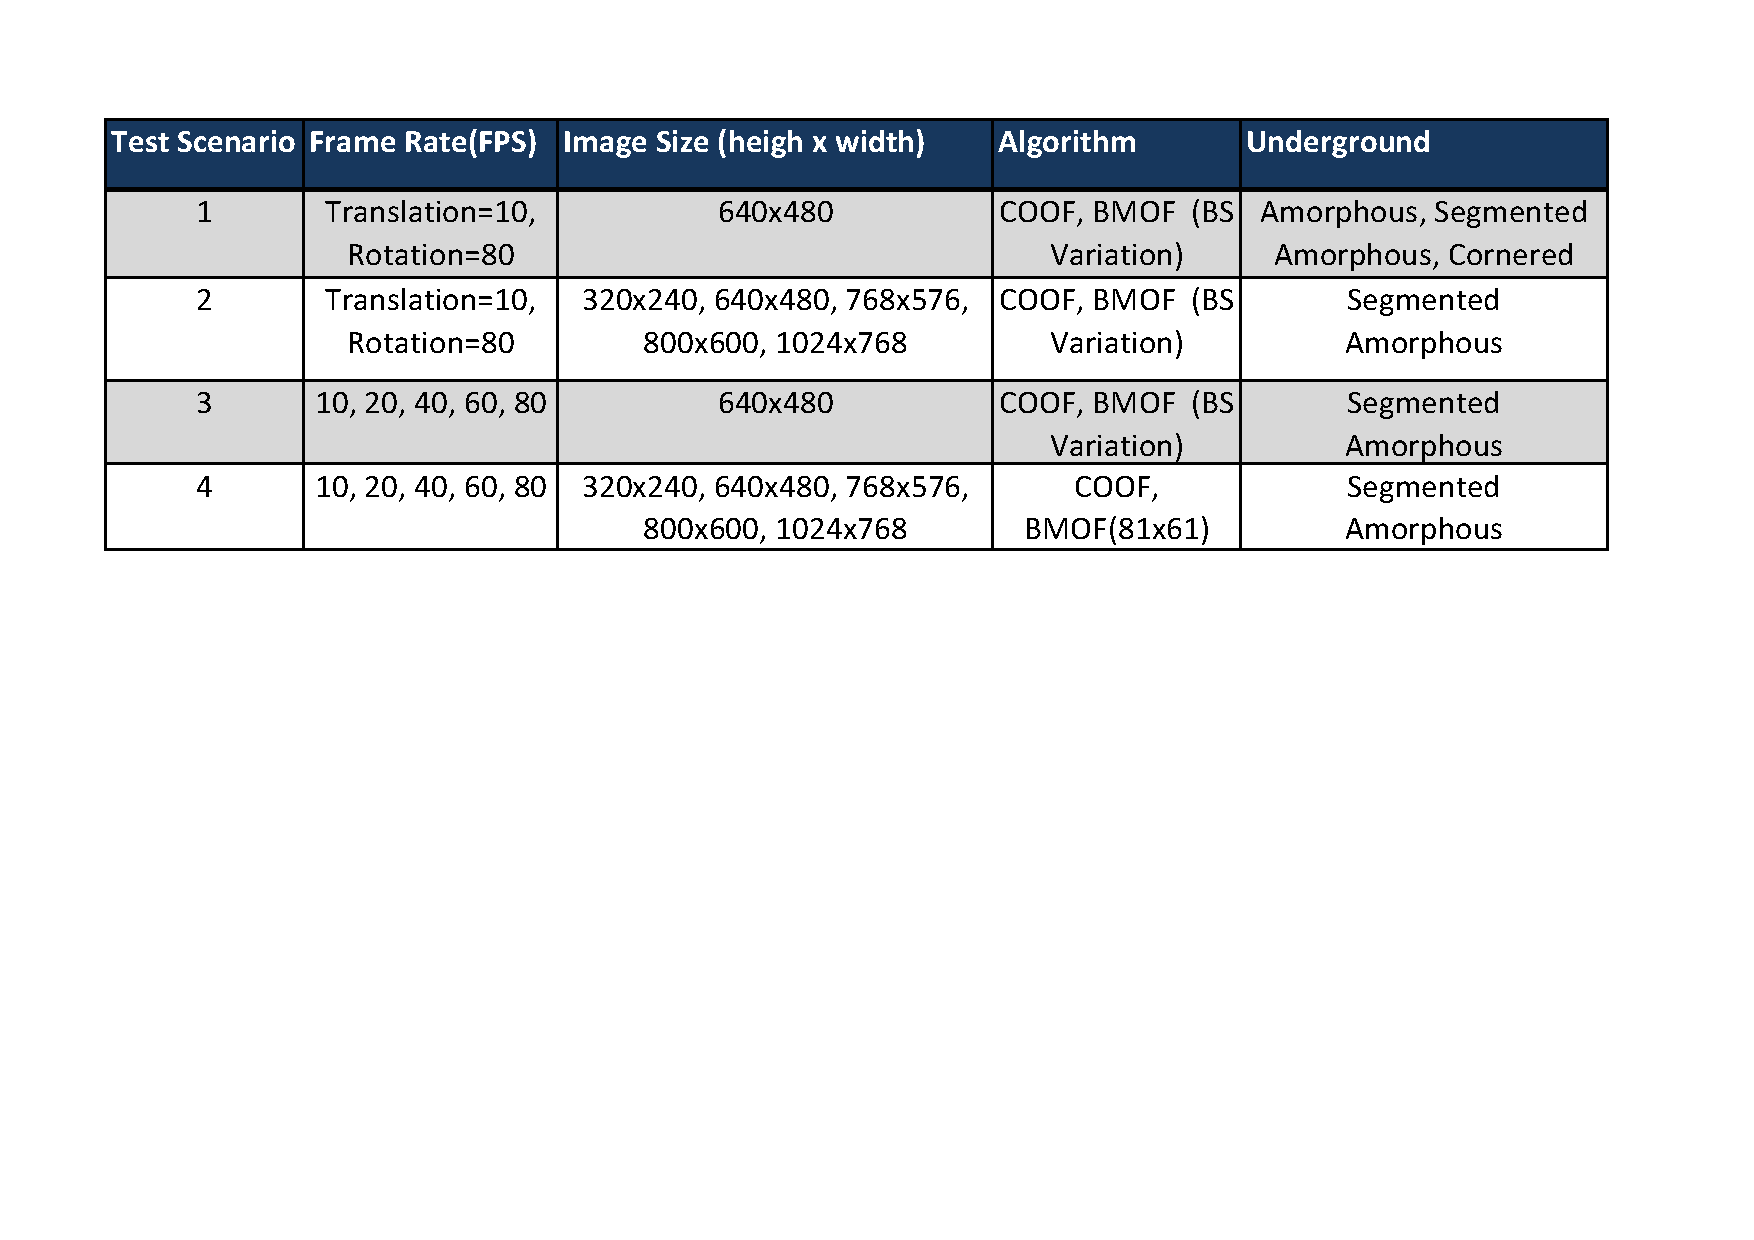
\includegraphics[width=1\textwidth]{graphic/ImageProcessingTestScenarioConfigurationValues.pdf}
	\caption{Image Processing test scenario configuration values}
	\label{fig:ImageProcessingTestScenarioConfigurationValues}
\end{figure}

%\begin{table}
%\begin{tabular}{|p{1cm}|p{5cm}|p{4cm}|p{2.5cm}|p{2.5cm}|}
%\hline
 %Test Scenario & FPS & Image Size & Algorithm & Underground\\
%\hline
%\hline
 %1 & Translation=10 FPS, Rotation=80FPS & 640x480 & COOF, BMOF(BS Variation) & Amorphous, Segmented Amorphous, Cornered\\
%\hline
 %2 & Translation=10 FPS, Rotation=80FPS & 320x240, 640x480, 768x576, 800x600, 1024x768 & COOF, BMOF(BS Variation) &Segmented Amorphous\\
%\hline
 %3 & 10, 20, 40, 60, 80 FPS &  640x480 & COOF, BMOF(BS Variation) &Segmented Amorphous\\
%\hline
 %4 & 10, 20, 40, 60, 80 FPS &  320x240, 640x480, 768x576, 800x600, 1024x768 & COOF, BMOF(81x61) &Segmented Amorphous\\
%\hline
%\hline
%\label{fig:ImageProcessingTestScenarioConfigurationValues}
%\end{tabular}
%\caption{Image Processing Test Scenario Configuration Values}
%\end{table}